\section{Modelli computazionali}

Prima di definire l'architettura del sistema, è stato necessario analizzare i diversi modelli computazionali delle tecnologie utilizzate al fine di effettuare una coerente integrazione tra i sistemi utilizzati. 

\subsection{JaCaMo}

\subsubsection{Jason - BDI Agent Model}

Gli agenti rappresentano l'astrazione principale dei MAS: sono entità proattive che incapsulano il controllo, governandolo attraverso azioni che consentono all'agente stesso di perseguire i propri obiettivi (ovvero, ciò che vuole ottenere) usando e cambiando qualcosa nel mondo in cui sono immersi (percependo lo stato dell'ambiente e adattando le proprie azioni e il proprio comportamento in base ad esso). In questo senso, gli agenti sono situati, strettamente uniti con il contesto e l'ambiente circostante e, cosa più importante, sono sociali: esprimono autonomia nelle interazioni tra agenti, come avviene in una società.

\medskip

Un particolare tipo di agente è quello presente in JaCaMo, sviluppato secondo l'architettura BDI. \'E possibile, e abbastanza comune, pensare ad un agente BDI come un sistema razionale con atteggiamenti mentali \cite{rao1995bdi}, vale a dire credenze (Beliefs), desideri (Desires), e intenzioni (Intentions), le quali rappresentano rispettivamente ciò che l'agente conosce del mondo, cosa lo motiva e cosa sta facendo per raggiungere i propri obiettivi. Come proposto in \cite{rao1995bdi}, il ciclo di reasoning di un agente è composto da quattro fasi principali:

\begin{enumerate}
    \item Generazione di opzioni: l'agente restituisce un insieme di opzioni in base a cosa conosce riguardo al mondo e quali sono i suoi desideri;
    \item Deliberazione: l'agente seleziona un sottoinsieme delle opzioni precedentemente selezionate;
    \item Esecuzione: l'agente esegue, se è presente la relativa intenzione, un'azione tra le opzioni precedentemente selezionate;
    \item Percezione: l’agente infine aggiorna la sua conoscenza del mondo (ed eventualmente sè stesso).
\end{enumerate}

\begin{figure}[H]
\centering
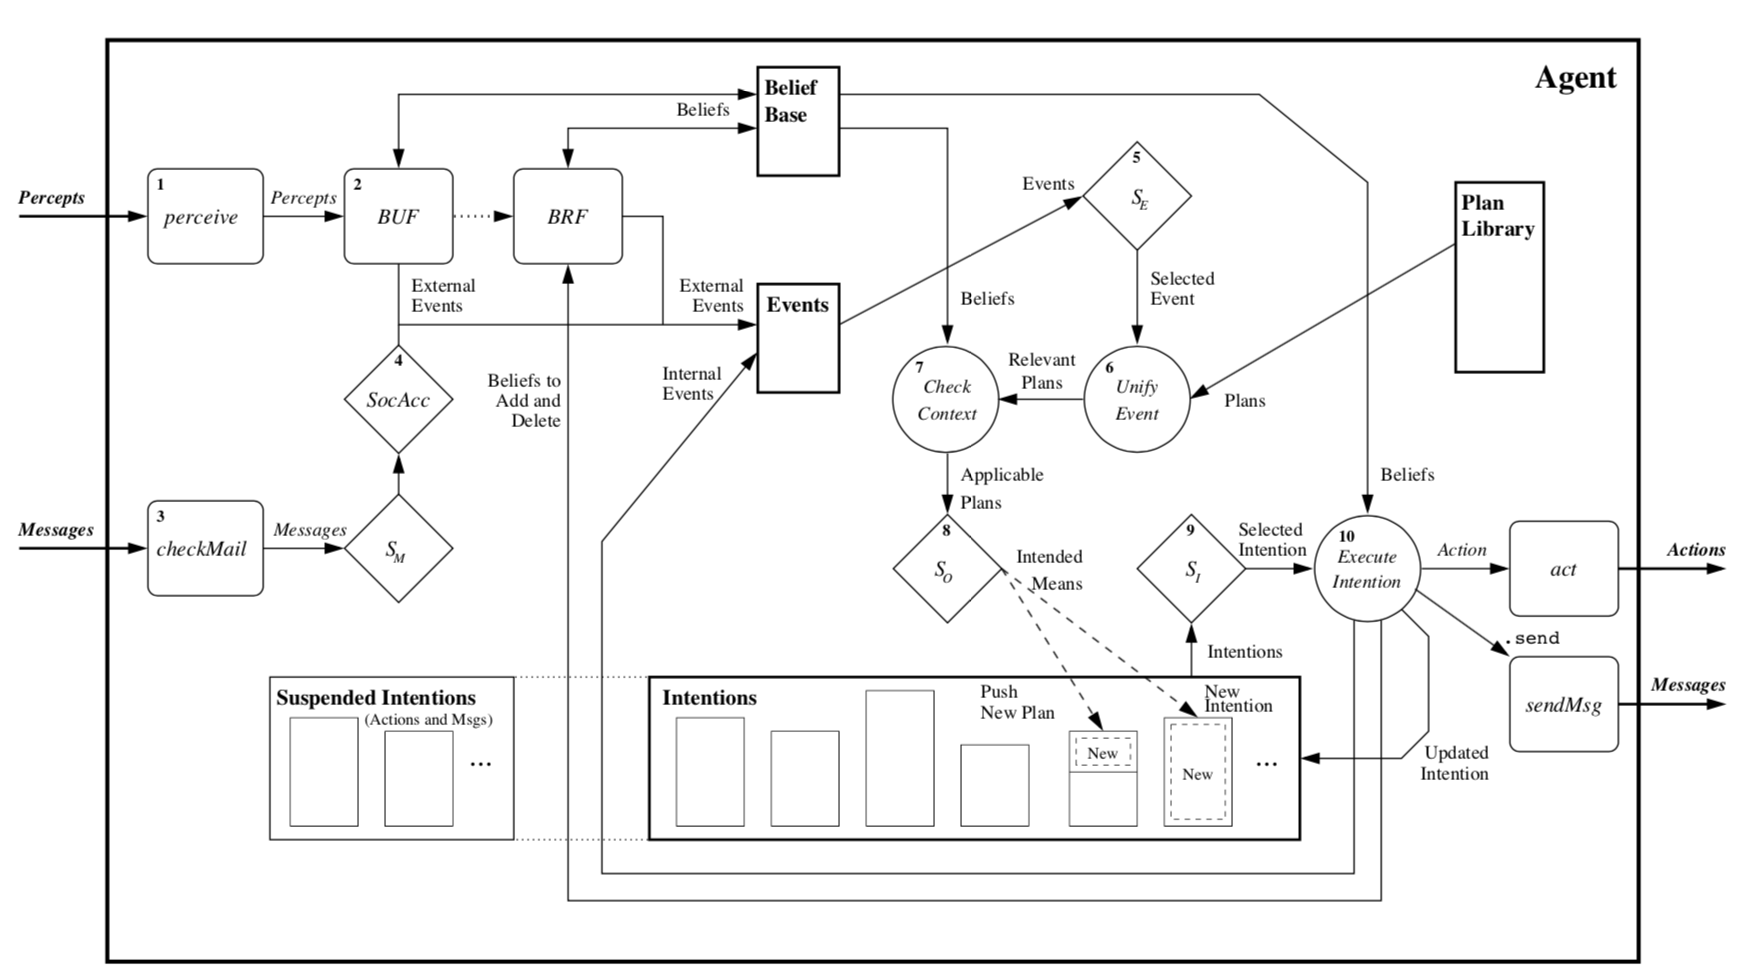
\includegraphics[width=\textwidth]{figures/Agent_BDI_Lifecycle.png}
\caption{Architettura BDI di un agente \cite{jason-book}}
\label{architettura_BDI_agente}
\end{figure}

Durante l'analisi delle astrazioni disponibili su Jason è risultato particolarmente utile il concetto di "belief". La Belief Base, raffigurata nell'immagine \ref{architettura_BDI_agente}, è il contenitore di conoscenza dell'agente che viene in parte modificata dalle percezioni esterne ricevute dall'ambiente. 

\medskip

Tali percezioni sono facilmente riconducibili agli eventi che un GameObject può ricevere durante la sua permanenza nell'ambiente (sezione \ref{ambiente_unity}), come, ad esempio la notifica di una collisione con un secondo GameObject in scena. Questo concetto ha portato alla decisione di utilizzare il belief come strumento per "notificare" all'agente le percezioni inviate dal GameObject.

\subsubsection{CArtAgO}

L'architettura astratta di CArtAgO (e degli ambienti di lavoro di CArtAgO) è composta da tre elementi costitutivi principali (vedi Fig. \ref{architettura_CArtAgO}): (i) corpi degli agenti - in quanto entità che rendono possibile situare agenti all'interno dell'ambiente di lavoro; (ii) artefatti: come elementi di base per strutturare l'ambiente di lavoro; e (iii) aree di lavoro, come contenitori logici di artefatti, utili per definire la topologia dell'ambiente di lavoro \cite{cartago}.

\begin{figure}[H]
\centering
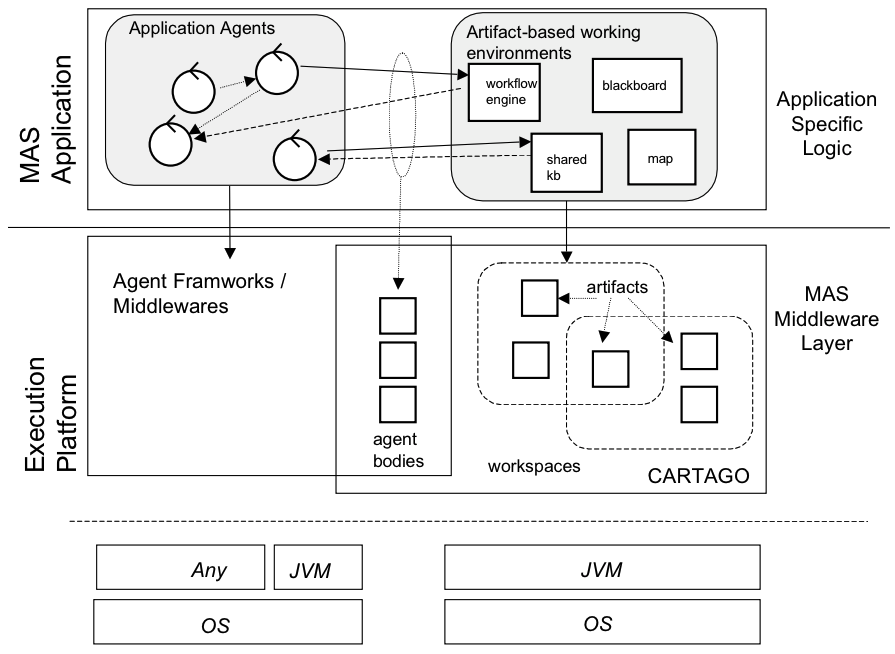
\includegraphics[width=\textwidth]{figures/CArtAgO_architettura.png}
\caption{Livelli del MAS che adottano il supporto CArtAgO. Gli ambienti applicativi sono modellati in termini di ambienti di lavoro basati su artefatti. Il middleware CArtAgO gestisce il ciclo di vita degli ambienti di lavoro, composto da artefatti raggruppati in aree di lavoro. I corpi degli agenti vengono utilizzati per collocarli all'interno degli ambienti di lavoro, eseguendo azioni su artefatto e percependo artefatti osservabili stato ed eventi \cite{cartago}.}
\label{architettura_CArtAgO}
\end{figure}

Analogamente ai manufatti nella nostra società, il modello di base che caratterizza l'interazione tra agenti e manufatti si basa su una nozione di uso e osservazione. Gli agenti possono utilizzare un artefatto innescando l'esecuzione delle operazioni elencate nell'interfaccia di utilizzo dell'artefatto. Un'operazione è caratterizzata da un nome e un insieme di parametri digitati. L'esecuzione di un'operazione provoca, in genere, l'aggiornamento dello stato interno di un artefatto e potenzialmente la generazione di uno o più eventi osservabili - comprese le condizioni di errore - che possono essere eventualmente raccolti dal sensore degli agenti quando vengono generati e percepiti attraverso azioni di rilevamento esplicite.

\medskip

L'artefatto è computazionalmente associabile al concetto di monitor. Un monitor è un costrutto di sincronizzazione di un linguaggio di alto livello. Un'istanza di un tipo monitor può essere utilizzata da due o più processi o thread per rendere mutuamente esclusivo l'accesso a risorse condivise. Il vantaggio nell'utilizzo del monitor deriva dal fatto che non si deve codificare esplicitamente alcun meccanismo per realizzare la mutua esclusione, giacché il monitor permette che un solo processo sia attivo al suo interno, imponendo la sequenzalizzazione delle azioni, che può essere limitante, ma serve a garantire consistenza dello stato interno del monitor.

\medskip

Analizzando le astrazioni disponibili su CArtAgO, i concetti di artefatto, "Observable Properties" e di "Operations" sono stati utili per l'integrazione con la Game Engine. L'immagine \ref{artifact_use} contiene un esempio di interazione tra agente ed artefatto dove viene fatto uso dei concetti precedentemente elencati.

\begin{figure}[H]
\centering
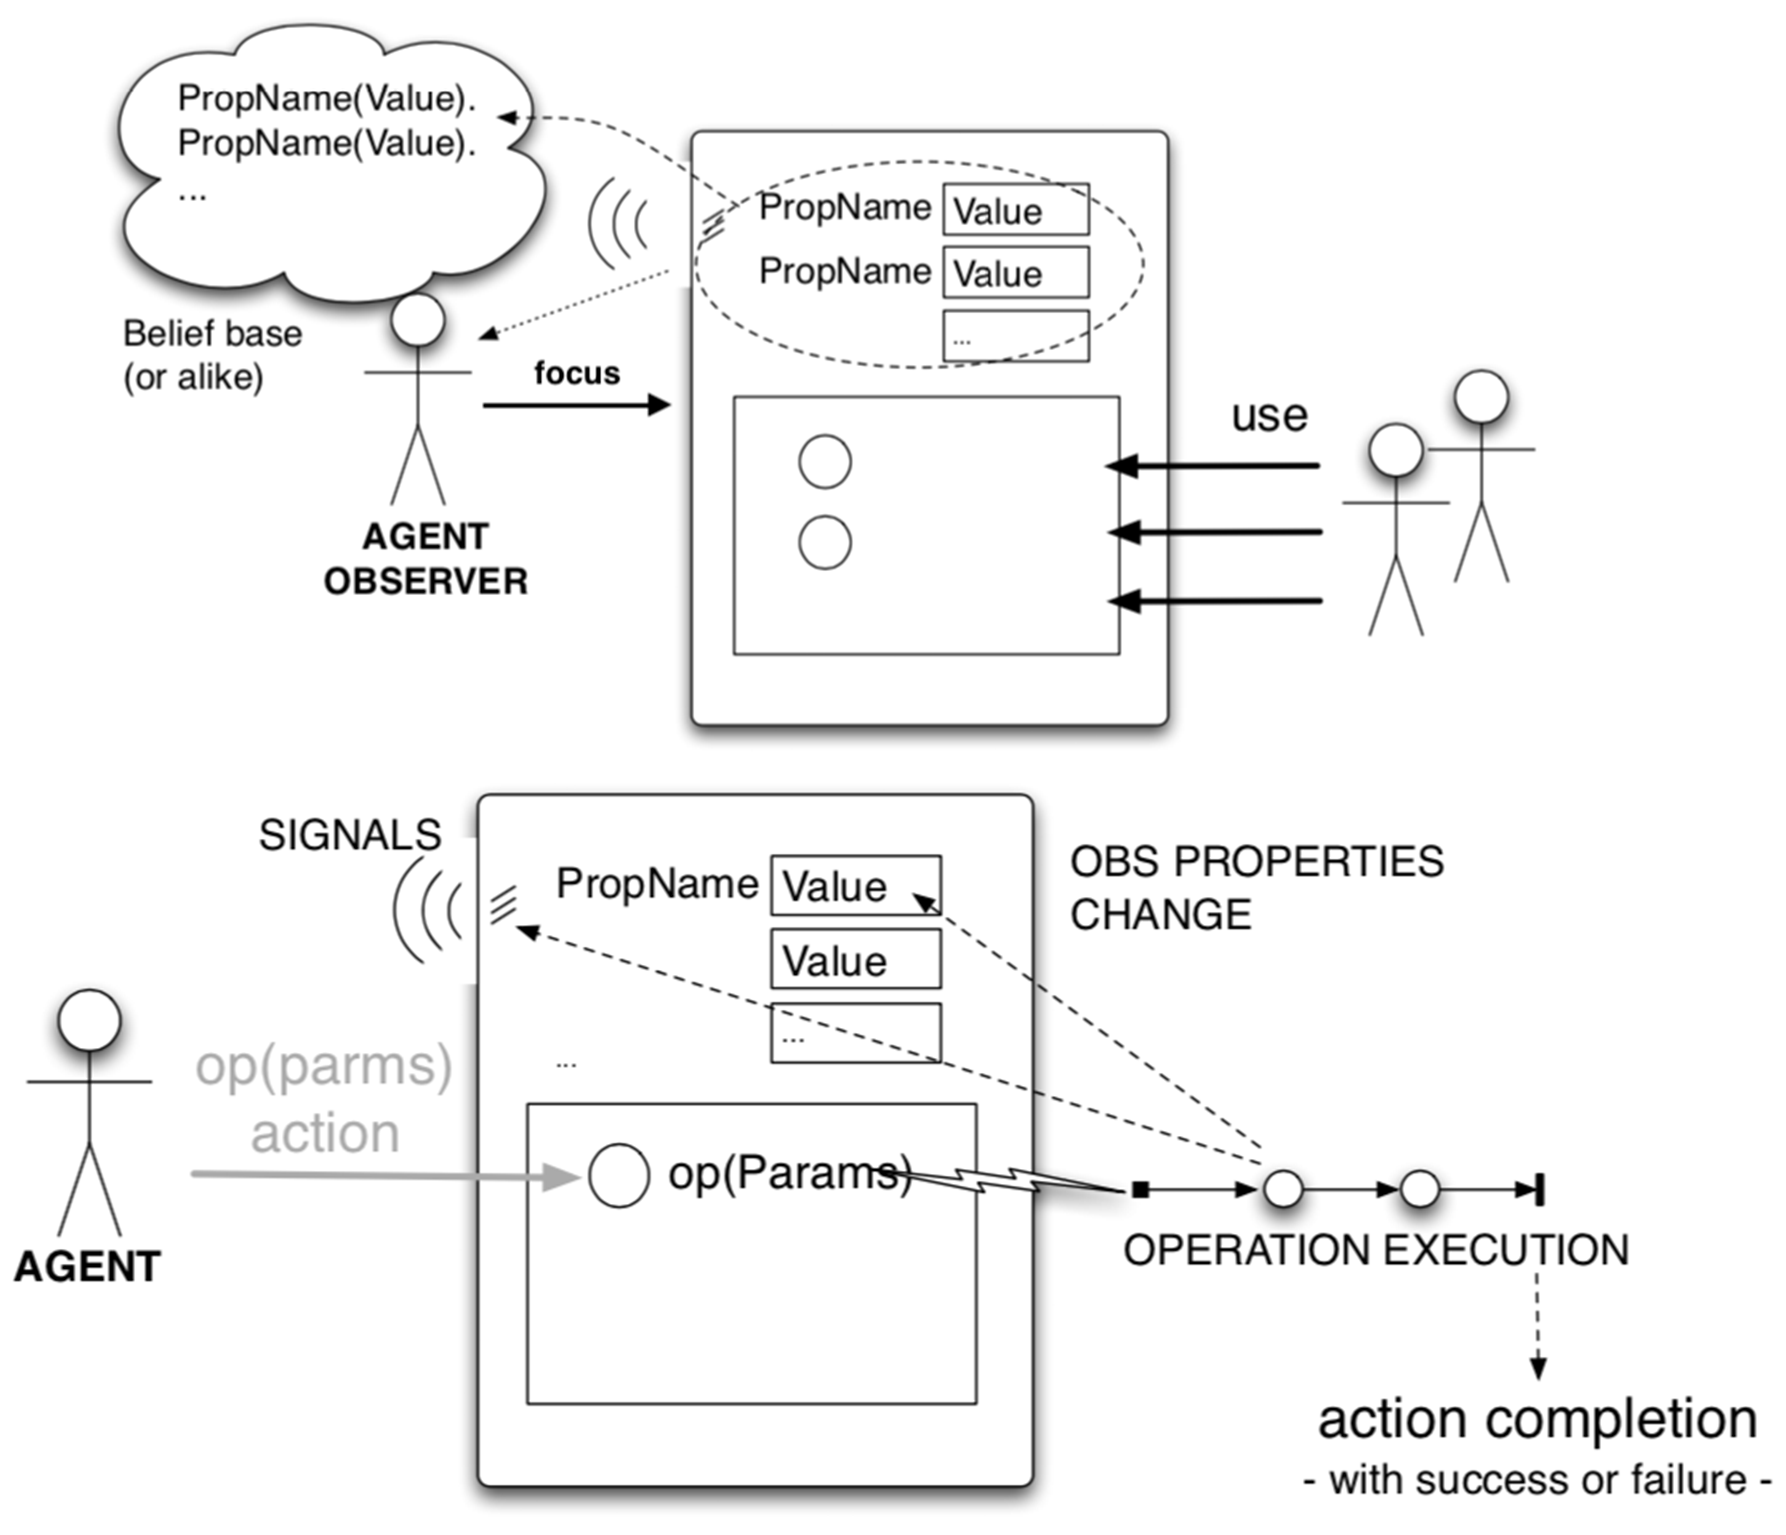
\includegraphics[width=0.8\linewidth]{figures/Artifact_use.png}
\caption{Interazione tra agente ed artefatto}
\label{artifact_use}
\end{figure}

L'artefatto ha contribuito a definire la principale modalità di integrazione tra JaCamo e Unity, dato che le sue finalità sono collegabili alle finalità di utilizzo del GameObject. Entrambi devono rappresentare una porzione di ambiente, risultare uno strumento a disposizione dell'agente per effettuare operazioni/azioni sull'ambiente e "notificare" l'agente in caso di modifiche sulle informazioni su essi contenute.

\begin{figure}[H]
\centering
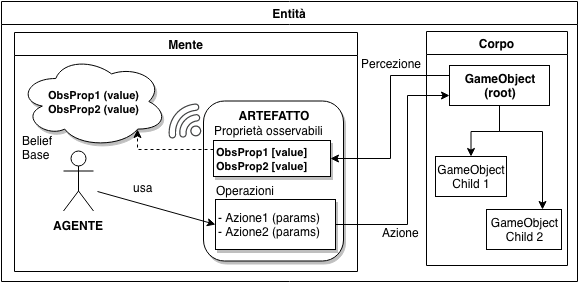
\includegraphics[width=\linewidth]{figures/Ridefinizione_entita.png}
\caption{Nuova struttura entità}
\label{struttura_nuova_entita}
\end{figure}

La definizione di queste associazioni tra Jason, CArtAgO e Unity ha portato ad una prima struttura delle componenti interne ad una generica entità, rappresentata nella figura \ref{struttura_nuova_entita}. \'E da notare la composizione del corpo: difatti, è stata lasciata la possibilità di strutturare il corpo utilizzando più GameObject con l'unico vincolo che solo la radice sia in grado di comunicare con la mente. 

\medskip

Per questo motivo è stato deciso di effettuare un'associazione 1:1 tra GameObject ed artefatto permettendo quindi al GameObject di inviare le proprie percezioni, ricevute dell'ambiente Unity sotto forma di eventi. Ciò è stato possibile utilizzando le proprietà osservabili dell'artefatto ed all'agente di effettuare azioni sul corpo attraverso le operazioni disponibili nell'artefatto. 

